\chapter{Computer Science Foundations}

\section{Introduction}

Computer science is the study of algorithms and data structures. Algorithms are step-by-step procedures for solving problems. Data structures are ways of organizing data so that it can be used efficiently. In this chapter, we will discuss some fundamental concepts in computer science, and how they relate to mathematics.

\section{Algorithms}

An algorithm is a step-by-step procedure for solving a problem. Algorithms can be written in many ways, but they all have the same basic structure. An algorithm consists of a sequence of steps, each of which is executed in turn. The steps may involve performing calculations, making decisions, or repeating a sequence of steps. The goal of an algorithm is to solve a specific problem, such as finding the shortest path between two points, or sorting a list of numbers.

Let's look at an example of an algorithm. The following algorithm adds 10 to a number:

\begin{lstlisting}
def add_ten(number):
    return number + 10

print(add_ten(5))  # Output: 15
\end{lstlisting}

This algorithm takes a number as input, adds 10 to it, and returns the result. We have not covered the syntax of Python yet so let's do so now.

\subsection{Syntax}

Python is a high-level programming language that is widely used in computer science. It is known for its simplicity and readability. That being said, it is important to understand the syntax of Python in order to write algorithms. Here are some basic concepts in Python:

\begin{itemize}
    \item \textbf{Variables}: Variables are used to store data. In Python, variables are created by assigning a value to a name. For example, \texttt{x = 5} creates a variable \texttt{x} and assigns it the value 5.
    \item \textbf{Functions}: Functions are blocks of code that perform a specific task. In Python, functions are defined using the \texttt{def} keyword. For example, \texttt{def add\_ten(number):} defines a function called \texttt{add\_ten} that takes a number as input.
        \begin{itemize}
            \item Functions can also return values. In Python, the \texttt{return} keyword is used to return a value from a function. For example, \texttt{return number + 10} returns the sum of the number and 10.
            \item Functions can also take multiple arguments. For example, \texttt{def add(x, y):} defines a function that takes two arguments.
        \end{itemize}
    \item \textbf{Indentation}: Python uses indentation to define blocks of code. Blocks of code are defined by the level of indentation. For example, the code inside a function definition is indented by four spaces.
    \item \textbf{Comments}: Comments are used to explain code. In Python, comments start with the \texttt{\#} symbol. For example, \texttt{\# This is a comment} is a comment.
    \item \textbf{Output}: The \texttt{print} function is used to output data. For example, \texttt{print(5)} outputs the number 5.
    \item \textbf{Input}: The \texttt{input} function is used to get input from the user. For example, \texttt{x = input("Enter a number: ")} gets a number from the user and stores it in the variable \texttt{x}.
    \item \textbf{Loops}: Loops are used to repeat a block of code. In Python, there are two types of loops: \texttt{for} loops and \texttt{while} loops. For example, \texttt{for i in range(5):} repeats a block of code five times.
    \item \textbf{Conditional statements}: Conditional statements are used to make decisions in code. In Python, conditional statements are defined using the \texttt{if}, \texttt{elif}, and \texttt{else} keywords. For example, \texttt{if x > 5:} makes a decision based on the value of \texttt{x}.
    \item \textbf{Lists}: Lists are used to store multiple items in a single variable. In Python, lists are created using square brackets. For example, \texttt{numbers = [1, 2, 3, 4, 5]} creates a list of numbers.
    \item \textbf{Dictionaries}: Dictionaries are used to store key-value pairs. In Python, dictionaries are created using curly braces. For example, \texttt{person = \{"name": "Alice", "age": 30\}} creates a dictionary of a person.
    \item \textbf{Sets}: Sets are used to store unique items. In Python, sets are created using curly braces. For example, \texttt{numbers = \{1, 2, 3, 4, 5\}} creates a set of numbers.
\end{itemize}

As we go through this chapter, we will expand on these concepts and show how they are used in algorithms. Let's start by looking at some basic algorithms.

\section{Basic Algorithms}

\subsubsection{Pythagorean Theorem}

The Pythagorean theorem states that in a right-angled triangle, the square of the length of the hypotenuse is equal to the sum of the squares of the lengths of the other two sides. In mathematical terms, if $a$ and $b$ are the lengths of the two sides of the triangle that form the right angle, and $c$ is the length of the hypotenuse, then:

\begin{equation}
    a^2 + b^2 = c^2 \quad \text{so} \quad c = \sqrt{a^2 + b^2}
\end{equation}

Let's write an algorithm that calculates the length of the hypotenuse given the lengths of the other two sides:

\begin{lstlisting}
# Finds the length of the hypotenuse given the lengths of the other two sides
# Args:
#     a: The length of one side of the triangle
#     b: The length of the other side of the triangle
# Returns:
#     The length of the hypotenuse

import math  # Import the math module for the square root function

def hypotenuse(a, b):
    return math.sqrt(a**2 + b**2)

print(hypotenuse(3, 4))  # Output: 5.0
\end{lstlisting}

This algorithm takes the lengths of the two sides of a right-angled triangle as input, calculates the square of each side, adds them together, takes the square root of the sum, and returns the result. The \texttt{math} module is used to access the square root function.

\subsubsection{Factorial}

The factorial of a non-negative integer $n$ is the product of all positive integers less than or equal to $n$. It is denoted by $n!$. For example, $5! = 5 \times 4 \times 3 \times 2 \times 1 = 120$. The factorial of 0 is defined to be 1.

Let's write an algorithm that calculates the factorial of a number:

\begin{lstlisting}
# Calculates the factorial of a number
# Args:
#     n: The number to calculate the factorial of
# Returns:
#     The factorial of the number

def factorial(n):
    for i in range(1, n):
        n *= i
    return n

print(factorial(5))  # Output: 120
\end{lstlisting}

This algorithm takes a number as input, multiplies it by all positive integers less than itself, and returns the result. The \texttt{range} function is used to generate a sequence of numbers from 1 to $n$. The algorithm uses a \texttt{for} loop to multiply the number by each element in the sequence. You may notice that the \texttt{range} function generates numbers from 1 to $n-1$. This is because the \texttt{for} loop starts at 1, and the multiplication is done in the loop. The \texttt{*=} operator is a shorthand for multiplying a variable by a value and assigning the result to the variable.

\subsubsection{Fibonacci Sequence}

The Fibonacci sequence is a series of numbers in which each number is the sum of the two preceding ones. It starts with 0 and 1. The sequence goes: 0, 1, 1, 2, 3, 5, 8, 13, 21, and so on. The $n$th term of the Fibonacci sequence can be calculated using the formula:

\begin{equation}
    F_n = F_{n-1} + F_{n-2}
\end{equation}
\newpage % Start the code snippet on a new page to avoid splitting it across pages

Let's write an algorithm that calculates the $n$th term of the Fibonacci sequence:


\begin{lstlisting}
# Calculates the nth term of the Fibonacci sequence
# Args:
#     n: The term to calculate
# Returns:
#     The nth term of the Fibonacci sequence

def fibonacci(n):
    if n == 0:
        return 0
    elif n == 1:
        return 1
    else:
        return fibonacci(n-1) + fibonacci(n-2)

print(fibonacci(5))  # Output: 5
\end{lstlisting}

This algorithm takes a number as input, and calculates the $n$th term of the Fibonacci sequence using a recursive function. The \texttt{if} and \texttt{elif} statements are used to handle the base cases of the sequence, which are 0 and 1. The algorithm calls itself with $n-1$ and $n-2$ to calculate the $n$th term.

\section{Data Structures}

Data structures are ways of organizing data so that it can be used efficiently. There are many different types of data structures, each with its own strengths and weaknesses. In this section, we will discuss some common data structures and how they are used in computer science.

\subsection{Arrays}

An array is a collection of elements, each identified by at least one array index or key. Arrays are used to store multiple items in a single variable. In Python, arrays are created using square brackets. For example, \texttt{numbers = [1, 2, 3, 4, 5]} creates an array of numbers.

In mathematics, an array is a rectangular arrangement of numbers, symbols, or expressions in rows and columns. For example, a matrix is a two-dimensional array of numbers. Matrices are used in many areas of mathematics, such as linear algebra and calculus. Let's look at an example of a matrix:

\begin{equation}
    A = \begin{bmatrix}
        1 & 2 & 3 \\
        4 & 5 & 6 \\
        7 & 8 & 9
    \end{bmatrix}
\end{equation}

This matrix has three rows and three columns. The element in the first row and first column is 1, the element in the second row and third column is 6, and so on. The elements of a matrix can be accessed using row and column indices. For example, $A_{2,3}$ is the element in the second row and third column of the matrix $A$. In this case, $A_{2,3} = 6$. Let's write an algorithm that accesses the elements of a matrix:

\begin{lstlisting}
# Accesses the element of a matrix
# Args:
#     matrix: The matrix to access
#     row: The row index of the element
#     col: The column index of the element
# Returns:
#     The element of the matrix at the specified row and column

def access_element(matrix, row, col):
    return matrix[row][col]

matrix = [[1, 2, 3], [4, 5, 6], [7, 8, 9]]
print(access_element(matrix, 1, 2))  # Output: 6
\end{lstlisting}

This algorithm takes a matrix and row and column indices as input, and returns the element of the matrix at the specified row and column. The algorithm uses the row index to access the row of the matrix, and the column index to access the element of the row. There is a package called NumPy that is commonly used for working with arrays and matrices in Python. NumPy provides many functions for creating, manipulating, and performing operations on arrays and matrices. Let's look at an example of using NumPy to create a matrix:

\begin{lstlisting}
import numpy as np  # Import the NumPy package

# Create a matrix using NumPy
matrix = np.array([[1, 2, 3], [4, 5, 6], [7, 8, 9]])

print(matrix)  # Output: [[1 2 3]
              #          [4 5 6]
              #          [7 8 9]]
\end{lstlisting}

This code snippet imports the NumPy package and creates a matrix using the \texttt{np.array} function. The matrix is then printed to the console. NumPy provides many functions for creating matrices, such as \texttt{np.zeros}, \texttt{np.ones}, and \texttt{np.random}. NumPy also provides functions for performing operations on matrices, such as addition, subtraction, multiplication, and division.

\subsection{Linked Lists}

A linked list is a linear data structure in which elements are stored in nodes. Each node contains a data element and a reference to the next node in the sequence. Linked lists are used to store collections of items that need to be accessed sequentially. There are many different types of linked lists, such as singly linked lists, doubly linked lists, and circular linked lists.

In mathematics, a linked list is a sequence of numbers, symbols, or expressions that are connected by links. For example, a polynomial is a linked list of terms, each of which contains a coefficient and an exponent. Polynomials are used in many areas of mathematics, such as algebra and calculus. Let's look at an example of a polynomial:

\begin{equation}
    P(x) = 3x^2 + 2x + 1
\end{equation}

This polynomial has three terms: $3x^2$, $2x$, and $1$. The coefficient of the first term is 3, the exponent is 2, and so on. The terms of a polynomial can be accessed using the coefficient and exponent. For example, the coefficient of the second term is 2, and the exponent is 1. Let's write an algorithm that accesses the terms of a polynomial:

\begin{lstlisting}
# Accesses the term of a polynomial
# Args:
#     polynomial: The polynomial to access
#     coefficient: The coefficient of the term
#     exponent: The exponent of the term
# Returns:
#     The term of the polynomial with the specified coefficient and exponent

def access_term(polynomial, coefficient, exponent):
    for term in polynomial:
        if term["coefficient"] == coefficient and term["exponent"] == exponent:
            return term

polynomial = [{"coefficient": 3, "exponent": 2},
              {"coefficient": 2, "exponent": 1},
              {"coefficient": 1, "exponent": 0}]
print(access_term(polynomial, 2, 1))  # Output: {"coefficient": 2, "exponent": 1}
\end{lstlisting}

This algorithm takes a polynomial and coefficient and exponent values as input, and returns the term of the polynomial with the specified coefficient and exponent. The algorithm uses a \texttt{for} loop to iterate over the terms of the polynomial, and an \texttt{if} statement to check if the coefficient and exponent of each term match the specified values.

\subsection{Trees}

A tree is a hierarchical data structure in which elements are stored in nodes. Each node contains a data element and references to its children nodes. Trees are used to store collections of items that need to be organized in a hierarchical manner. There are many different types of trees, such as binary trees, binary search trees, and AVL trees.

In mathematics, a tree is a connected graph with no cycles. Trees are used to represent relationships between objects, such as family trees and organizational charts. For example, a family tree is a tree that represents the relationships between family members. Let's look at an example of a family tree:


\begin{figure}[H]
    \centering
    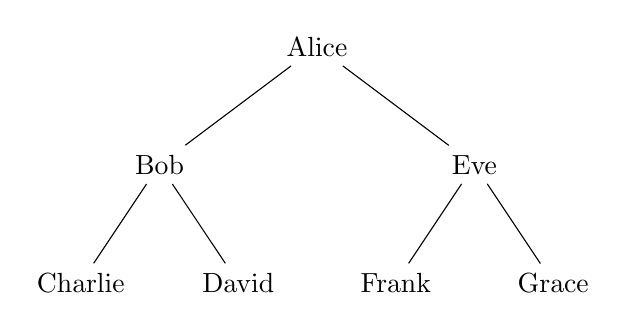
\begin{tikzpicture}[
      level 1/.style={sibling distance=40mm},  % Adjust the distance between siblings in level 1
      level 2/.style={sibling distance=20mm}   % Adjust the distance between siblings in level 2
    ]
        \node {Alice}
            child {node {Bob}
                child {node {Charlie}}
                child {node {David}}
            }
            child {node {Eve}
                child {node {Frank}}
                child {node {Grace}}
            };
    \end{tikzpicture}
    \caption{Family Tree}\label{fig:family-tree}
\end{figure}


This family tree has four generations: Alice, Bob, Charlie, David, Eve, Frank, and Grace. Alice is the parent of Bob and Eve, Bob is the parent of Charlie and David, and so on. The relationships between family members can be represented using a tree structure. Let's write an algorithm that accesses the children of a node in a family tree:

\begin{lstlisting}
# Accesses the children of a node in a family tree
# Args:
#     tree: The family tree to access
#     node: The node to access
# Returns:
#     The children of the node in the family tree

def access_children(tree, node):
    for parent, children in tree.items():
        if parent == node:
            return children

tree = {"Alice": ["Bob", "Eve"],
        "Bob": ["Charlie", "David"],
        "Eve": ["Frank", "Grace"]}
print(access_children(tree, "Bob"))  # Output: ["Charlie", "David"]
\end{lstlisting}

\newpage % Start the code snippet on a new page to avoid splitting it across pages

\section{Conclusion on Computer Science Foundations}

In this chapter, we discussed some fundamental concepts in computer science, such as algorithms and data structures. Algorithms are step-by-step procedures for solving problems, and data structures are ways of organizing data so that it can be used efficiently. We looked at some basic algorithms, such as the Pythagorean theorem, factorial, and Fibonacci sequence. We also discussed some common data structures, such as arrays, linked lists, and trees. These concepts are essential for understanding computer science and its applications in mathematics.
